\chapter{La chaîne de calcul en un coup d'œil}
\label{chap:chaine}

\begin{chapeau}
Ce chapitre donne la carte de la partie II : les étapes, les fichiers qu'elles échangent, les repères dans lesquels
on calcule, les données du projet et les hypothèses de travail.
\end{chapeau}

\section{Les étapes et les fichiers}

La \cref{fig:chaine-complete} montre le chemin d'un cas. Les étapes 1 à 6 sont écrites en Python (dossier
\fichier{code_source/}). La planification CORA est écrite en JavaScript et tourne dans la fenêtre de l'application ;
elle produit une \emph{prescription}, un fichier JSON qui dit où couper et comment corriger. L'étape 7, de nouveau en
Python, transforme cette prescription en guides imprimables.

\begin{figure}[htbp]
\centering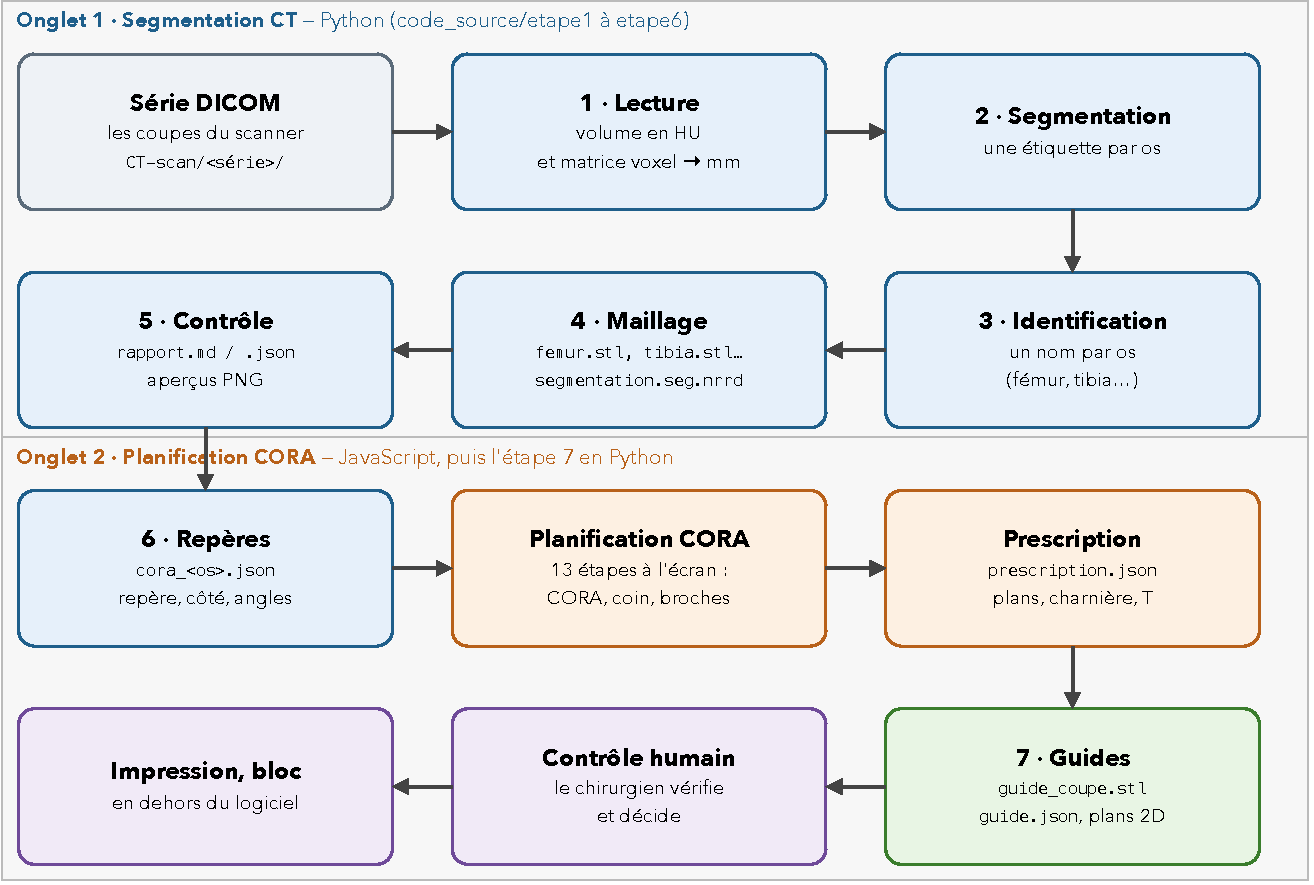
\includegraphics[width=\linewidth]{chaine_complete.pdf}
\caption{La chaîne complète : étapes, programmes et fichiers échangés.}
\label{fig:chaine-complete}
\end{figure}

\begin{table}[htbp]
\centering\small
\caption{Les étapes, leurs entrées, leurs sorties et leur durée (Mac Apple M5, 16~Go de mémoire).}
\label{tab:etapes}
\begin{tabularx}{\linewidth}{L{2.5cm}L{3.1cm}Y L{1.9cm}}
\toprule
\titrecol{Étape} & \titrecol{Fichier du code} & \titrecol{Ce qu'elle produit} & \titrecol{Durée} \\
\midrule
1 · Lecture & \fichier{etape1_lecture_dicom.py} & volume en HU et matrice voxel → millimètres & quelques s \\
2 · Segmentation & \fichier{etape2_segmentation.py} & une étiquette (un numéro) par os & 10 à 40 s \\
3 · Identification & \fichier{etape3_identification.py} & un nom par os ; tête du fémur & quelques s \\
4 · Maillage & \fichier{etape4_maillage.py} & un STL étanche par os, \fichier{segmentation.seg.nrrd} & 10 à 30 s \\
5 · Contrôle & \fichier{etape5_controle.py} & sensibilité au seuil, aperçus, \fichier{rapport.md} et \fichier{.json} & 10 à 40 s \\
6 · Repères & \fichier{etape6_reperes.py} & \fichier{cora_<os>.json} : repère, côté, repères, angles & 1,3 s par os \\
Planification & \fichier{cora/app/cora_simple.js} & \fichier{prescription.json} & instantané \\
7 · Guides & \fichier{etape7_guide.py}, \fichier{dessin_guide.py} & STL à imprimer, \fichier{guide.json}, plans 2D & 11 à 31 s \\
\bottomrule
\end{tabularx}
\end{table}

Les étapes 1 à 6 se lancent ensemble (bouton \ui{Segmenter la série} de l'application, ou
\fichier{lancer_tout.py} en ligne de commande) : de 25~s pour le pied à 2~min pour la série hanche--genou du lévrier.
Tout ce qui est produit pour un scanner va dans \fichier{resultats/<série>/}.

\begin{pourquoi}
\textbf{Pourquoi deux langages ?} Les calculs lourds (images de 200 millions de voxels, maillages, opérations
booléennes) demandent les bibliothèques scientifiques de Python. La planification, elle, doit réagir tout de suite
quand on bouge un curseur et s'afficher en 3D : elle tourne donc dans la page, en JavaScript, avec Three.js pour la
3D. Les deux parties ne partagent que des fichiers (JSON et maillages binaires) : chacune peut être testée seule.
\end{pourquoi}

\section{Les repères}
\label{sec:repere-os}

Trois repères se succèdent.

\textbf{1. Les indices de voxels} $(i, j, k)$ : colonne, ligne et numéro de coupe dans le volume. C'est le repère
du tableau numpy, stocké dans l'ordre $(k, j, i)$.

\textbf{2. Le repère du scanner}, LPS, en millimètres (\cref{sec:scanner}). Une matrice $4 \times 4$, notée
$\mt{A}$, passe des indices aux millimètres (\cref{sec:affine}). Les STL des os sont écrits dans ce repère : ils se
superposent exactement au scanner dans 3D Slicer.

\textbf{3. Le repère de l'os}, propre à chaque fémur ou tibia : $X$ latéral, $Y$ proximal, $Z$ caudal ; origine au
centre de l'articulation distale, au niveau du bout distal de l'os. Il est construit par l'étape 6
(\cref{sec:repere-construction}). Toute la planification et la construction des guides se font dans ce repère.

Le passage du scanner à l'os est une transformation rigide, éventuellement précédée d'un miroir :
\begin{equation}
  \vb{p}_{\text{os}} = \mt{R}\,(\mt{S}\,\vb{p}_{\text{scanner}} - \vb{o}),
  \qquad
  \mt{S} = \begin{cases} \mt{I} & \text{membre droit,} \\ \operatorname{diag}(-1, 1, 1) & \text{membre gauche,} \end{cases}
  \label{eq:repere-os}
\end{equation}
où les lignes de $\mt{R}$ sont les directions $X$, $Y$, $Z$ de l'os (dans le repère du scanner, après miroir) et
$\vb{o}$ son origine. Le logiciel l'écrit sous forme d'une matrice $4 \times 4$ dans \fichier{cora_<os>.json}
(clé \code{scanner_vers_os}). Son déterminant vaut $-1$ quand le membre a été mis en miroir.

\begin{attention}[title={Le miroir retourne les triangles}]
Un miroir change l'orientation de l'espace : un triangle $(a, b, c)$ dont la normale sortait de l'os la ferait
rentrer. Après un miroir, le logiciel inverse donc l'ordre des sommets de chaque triangle, $(a, c, b)$, pour garder
des normales sortantes (fonction \code{miroir_maillage()} de l'étape 6, et \code{maillage_dans_repere()}).
\end{attention}

\section{Les données du projet}
\label{sec:donnees}

\subsection{Les scanners du lévrier}

Le projet dispose de trois scanners d'un lévrier sain, réalisés sur un GE LightSpeed Ultra (120~kV, noyau
« BONEPLUS ») : hanche--genou (728 coupes), genou--cheville (748 coupes) et pied (442 coupes), toutes de 0,625~mm, en
images de $512 \times 512$ pixels de 0,27 à 0,56~mm. Les trois séries sont trois examens distincts. Le fémur complet
est dans la série hanche--genou, le tibia complet dans la série genou--cheville ; les autres fémurs et tibias sont
coupés par le bord du champ et sont refusés pour la méthode CORA (\cref{sec:completude}).

\subsection{L'os fictif}

Pour tester la planification sur un os parfaitement connu, le projet utilise aussi un \textbf{os fictif} : un fémur,
un tibia et une fibula de chien d'environ 30~kg, fabriqués par ordinateur (\fichier{code_source/cora/generate_bones.py}).
Chaque os est une somme lisse de formes simples (sphères, ellipsoïdes, cônes arrondis) décrites par des fonctions de
distance, puis transformée en maillage par marching cubes. Ses repères anatomiques sont connus exactement, et ses
angles sont réglés sur les valeurs publiées (aLPFA 103\degre, aLDFA 97\degre, mMPTA 93,4\degre, mMDTA 96,3\degre,
mCaPTA 63,8\degre, mCrDTA 81,7\degre, antéversion d'environ 31\degre).

\subsection{Les déformités simulées}

Un os sain ne demande pas de correction. Pour tester le logiciel, on lui impose une \textbf{déformité connue}
(\cref{sec:deformite-simulee}) : le segment distal tourne d'un angle choisi autour d'un axe passant par l'apex, avec
éventuellement une torsion. Comme on connaît la réponse, on mesure l'erreur exactement. C'est le niveau 1 de la
validation (\cref{chap:validation}).

\section{Les hypothèses de travail}
\label{sec:hypotheses}

Ce sont les choix faits pour que le projet reste réalisable. Les résultats ne valent que dans ce cadre.
\begin{enumerate}
  \item Un scanner du membre est disponible, avec des coupes de 1~mm ou moins.
  \item La surface d'os trouvée par le logiciel est à moins de 0,5~mm de la vraie surface (vérifié au
  \cref{chap:maillage}).
  \item Chaque os est fait de deux segments droits autour d'\textbf{une seule} zone tordue (un seul apex).
  \item \textbf{Fémur : seulement les déformités distales}, apex entre 62 et 82~\% de la longueur depuis le haut.
  Les déformités du col (coxa vara ou valga, antéversion) se corrigent par une autre ostéotomie et sortent du projet.
  Au tibia, l'apex peut être entre 25 et 85~\%.
  \item La référence est le membre opposé sain, ou à défaut les valeurs normales publiées.
  \item L'os est rigide, et la correction se fait en une fois pendant l'opération.
  \item Les muscles, les ligaments et la plaque ne sont pas modélisés.
  \item Seulement des coupes planes (pas de dôme) ; l'angle et la torsion sont corrigés par un coin suivi d'une
  rotation.
  \item Le chien est adulte par défaut (une option existe pour un chien en croissance).
  \item Les voies d'abord et les marges de sécurité sont des choix raisonnés, à valider avec un chirurgien.
\end{enumerate}

\section{Les bibliothèques utilisées}

Le logiciel n'utilise que des outils gratuits et libres (\cref{tab:bibliotheques}). Ils sont installés une fois par
les lanceurs (\cref{sec:lancer}) ou copiés dans l'application autonome.

\begin{table}[htbp]
\centering\small
\caption{Les bibliothèques et leur rôle.}
\label{tab:bibliotheques}
\begin{tabularx}{\linewidth}{L{3.1cm}YL{2.4cm}}
\toprule
\titrecol{Outil} & \titrecol{Rôle dans le projet} & \titrecol{Licence} \\
\midrule
Python 3.10 et plus & langage des calculs & PSF \\
numpy, scipy \cite{harris2020,virtanen2020} & tableaux, algèbre linéaire, morphologie, arbres k-d & BSD \\
pydicom & lecture des fichiers DICOM & MIT \\
SimpleITK \cite{lowekamp2013} & lissage, ligne de partage des eaux, cartes de distance & Apache 2.0 \\
VTK, pyvista \cite{schroeder2006} & isosurfaces, lissage et décimation de maillages, rendus & BSD, MIT \\
trimesh & maillages : contrôles, coupes, normales & MIT \\
manifold3d \cite{manifold} & opérations booléennes exactes des guides & Apache 2.0 \\
matplotlib & figures, plans 2D & type PSF \\
pywebview & fenêtre native de l'application & BSD \\
Three.js & affichage 3D dans l'interface & MIT \\
PyInstaller & fabrication de l'application autonome & GPL avec exception \\
\bottomrule
\end{tabularx}
\end{table}
